% stats.tex : appendix tutorial; python listings, 65 chars wide
\section{A Tutorial on Ranking Statistics}
\label{sec:stats}

\subsection{Why Argue with Distributions?}

Software engineering practices are highly variable: different
people use different tools on different platforms in pursuit of
different goals.
Reasoning about software engineering therefore means studying
not just average effects but also the variability around those
effects.
That variability has many sources.
Project data is noisy, since no two projects share the same
staff, toolchain, platform, or objectives.
Some of the ``data'' is really guesswork; e.g. when human
experts estimate the value of a tool or an industrial process.
Modeling adds more variance: learners shuffle their data,
optimizers roll dice, and large language models sample their
tokens.
The same data can hence yield many different models, and a
useful conclusion must hold across all those models, not just
one.
A single result is therefore not a fact but a lottery ticket,
and honest comparisons must argue with \textbf{distributions},
not points.
Two treatments whose result clouds overlap heavily are, for
practical purposes, the same treatment, no matter which one
``won'' on any single run.

The record shows the cost of skipping this step.
Cohen spent a career documenting how significance testing,
uncoupled from effect size, filled psychology with findings too
small to matter~\cite{cohen88,cohen94}.
Decades later, a mass replication of one hundred published
psychology studies confirmed barely more than a third of
them~\cite{osc15}.
Ioannidis argued that under low power and flexible analysis,
most published findings are simply false~\cite{ioannidis05};
Gelman and Loken traced the mechanism to the ``garden of
forking paths,'' where innocent analytic choices manufacture
significance~\cite{gelman14}.
Software engineering shows the same problem: a systematic
review found that most SE experiments did not report effect
sizes at all, so readers could not tell large results from
small ones~\cite{kampenes07}.
Such mistakes are costly; e.g. months of compute and writing
can be spent defending a one-percent improvement that no user
of the system would notice.

The fix is cheap.
Arcuri and Briand's practical guide for randomized algorithms
in SE offers much relevant advice; central to that advice is to
prefer non-parametric tests and to pair every significance test
with an effect size~\cite{arcuri11}.
This appendix implements our version of that advice, then
extends it from comparing two treatments to ranking many, all
in 44 lines of Python.

That last paragraph used three technical terms:
\begin{itemize}
\item a \textbf{significance test} asks whether a difference
  could plausibly be chance alone;
\item an \textbf{effect size} measures how big a difference is;
\item \textbf{non-parametric} methods rank or count, and assume
  no particular distribution shape.\footnote{As opposed to
  \emph{parametric} tests, which assume all values fit some
  idealized, but possibly unrealistic, curve such as the normal
  Gaussian.}
\end{itemize}
Throughout this appendix, statistical terms appear in
\textbf{bold} at their first use
(and are defined in Table~\ref{tbl:jargon}).

\begin{table}[t]
\caption{Statistical jargon used in this appendix.}
\label{tbl:jargon}
\small
\begin{tabular}{@{}p{0.2\linewidth}p{0.72\linewidth}@{}}
\toprule
term & meaning\\
\midrule
\textbf{sample} &
  The numbers actually collected; e.g. twenty repeated runs of
  one treatment.
  Samples stand in for the infinite population of runs that
  could have happened.\\
\textbf{distribution} &
  The shape of a sample: where its values pile up and how far
  they spread.\\
\textbf{mean, median} &
  Two centers of a distribution: the average, and the middle
  value after sorting.
  Medians resist outliers, so they suit skewed data.\\
\textbf{variance, standard deviation} &
  How far values scatter about the mean; the deviation is the
  square root of the variance, in the same units as the data.
  A \emph{pooled} deviation blends the spread of two samples,
  weighting each by its size.\\
\textbf{pdf} &
  The probability density function: for any value $v$, the
  fraction of the sample at $v$; i.e. the shape of the data.\\
\textbf{cdf} &
  The cumulative distribution function: for any value $v$, the
  fraction of the sample at or below $v$.
  A sorted list gives the cdf directly.\\
\textbf{significance test} &
  A check of whether a difference this large could plausibly
  arise by chance alone, given some tolerated false-alarm rate
  (often five percent).\\
\textbf{critical value} &
  The tabled cutoff a test statistic must exceed before a
  result counts as significant at a given false-alarm rate
  (often five percent).\\
\textbf{effect size} &
  How big a difference is, in units that survive translation
  between studies; e.g. ``half a standard deviation,'' not
  ``0.03 on our benchmark.''\\
\textbf{parametric, non-parametric} &
  Parametric tests assume a distribution shape (usually the
  bell curve); non-parametric tests rank or count instead, so
  they survive skew, ties, and outliers.\\
\textbf{rank} &
  A position after sorting.
  Statistics built on ranks use order, not magnitude, which
  makes them robust to skew, ties, and outliers.\\
\bottomrule
\end{tabular}
\end{table}

\subsection{A Worked Example}
\label{sec:worked}

To make this concrete, suppose three teams race to deliver a
first minimal viable product, each using a different agent
framework ($a$, $b$, $c$).
Each framework is tried twenty times; the outcome is the whole
number of days until that first MVP ships:

\begin{center}\ttfamily\footnotesize
\begin{tabular}{r@{~~}l}
a: & 1 2 2 2 3 3 3 3 3 4 4 4 4 5 5 5 6 6 7 8\\
b: & 5 6 6 7 7 7 8 8 8 8 8 9 9 9 9 10 10 10 11 11\\
c: & 5 6 6 7 7 8 8 8 8 9 9 9 9 9 10 10 10 11 11 11
\end{tabular}
\end{center}

Do these \textbf{samples} actually say different things?
Figure~\ref{fig:xdf} shows two views of the data.
The left-hand plot shows each sample's \textbf{probability
density function} (pdf); i.e. how the values are distributed
(so, e.g., $a$'s most common value is three days).
The right-hand plot shows what fraction of the projects
finished within a given number of days; this is called a
\textbf{cumulative distribution function} (cdf).
Intuitively, the answer seems clear: $b$ and $c$ pile up around
eight or nine days and overlap almost everywhere, while $a$
sits several days to their left.
The eye says $a$ is different and $b,c$ are the same.

An eyeball, however, is not an argument.
Reviewers will ask how much overlap counts as ``almost
everywhere,'' and whether four days is a large gap or a small
one.
The science of statistics is how to make defensible
conclusions from
distributions like those in Figure~\ref{fig:xdf}.
For an example of that kind of conclusion, see the rest of this
appendix.

\begin{figure}[t]
\centering
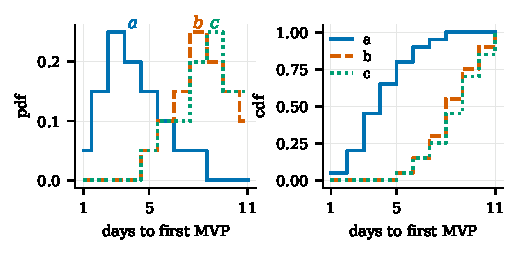
\includegraphics[width=.9\linewidth]{fig/stats_xdf}
\caption{Twenty runs per framework: days to first MVP, as
probability density functions (left) and cumulative
distribution functions (right).
Frameworks $b$ and $c$ overlap almost everywhere; $a$ is
several days faster.
Regenerate with \texttt{make statsfig}.}
\label{fig:xdf}
\end{figure}

\subsection{Two Questions, One Verdict}

Statistical comparisons answer two different questions.
A significance test asks: could a gap this large be chance?
An effect size asks: is the gap big enough to matter?
The two can disagree: given enough runs, even a microscopic
difference passes a significance test, while with too few runs,
even a large difference can be luck.
One check guards against noise, the other against triviality;
hence standard advice runs both~\cite{arcuri11}.

Our code adds one more safeguard.
Effect sizes come in parametric and non-parametric flavors, and
each can be fooled in its own way, so both flavors are run.
Two samples are called ``the same'' only when all three tests
agree that the difference is small: two effect sizes
(\texttt{cohen}, \texttt{cliffs}) and one significance test
(\texttt{ks}), each defined in the sections that follow.
Python's \texttt{and} is lazy, so the cheapest test runs first
and the costlier ones run only when needed.

Every test here expects sorted input; that one convention buys
linear scans, percentile tricks, and free medians throughout.
By default \texttt{same} trusts its caller to pre-sort (as
\texttt{ranks} does below); pass \texttt{is\_sorted=False}
and it sorts defensively first.

\begin{lstlisting}[style=py]
def same(xs, ys,
         c0=.35,   # cohen threshold; from |\cite{cohen88,sawilowsky09}|
         d0=.195,  # cliffs threshold; from |\cite{romano06}|
         k0=1.36,  # ks threshold; from |\cite{massey51}|
         is_sorted=True):
    if not is_sorted:
        xs, ys = sorted(xs), sorted(ys)
    return (cohen(xs, ys)  <= c0 and
            cliffs(xs, ys) <= d0 and
            ks(xs, ys)     <= k0)
\end{lstlisting}

On the worked example of \S\ref{sec:worked}, all three tests
agree:
\begin{itemize}
	\item
Comparing $b$ to $c$ yields $d\!=\!0.13$, $\delta\!=\!0.10$,
and $\mathit{ks}\!=\!0.32$: all under their thresholds, so
\texttt{same} returns true.
\item
Comparing $a$ to $b$ yields $d\!=\!2.2$, $\delta\!=\!0.91$, and
$\mathit{ks}\!=\!2.4$: all far over, so \texttt{same} returns
false.
\end{itemize}
Taken together, those verdicts divide the three frameworks into
two groups:
\begin{center}
\texttt{( (a), (b, c) )}
\end{center}
The eyeball intuition is now a defensible claim.

For code that reports these groupings, see 
\S\ref{sec:ranks}.

\subsection{Significance: the Kolmogorov--Smirnov Test}

\textbf{Means} can agree while distributions disagree; e.g.
two samples can share an average while one is tight and the
other is spread wide.
The Kolmogorov--Smirnov statistic guards against this by
comparing whole cumulative distributions~\cite{massey51}.
The intuition runs as follows.
If two samples come from the same source, their cdfs should
ride on top of each other: at every value, about the same
fraction of each sample lies below.
Anywhere the curves pull far apart, one treatment has finished
far more of its runs than the other, so the distributions must
differ.

The KS statistic reports the  largest vertical gap between cdfs.
For example,
Figure~\ref{fig:ks} repeats the cdfs of
Figure~\ref{fig:xdf}, now with that gap drawn in
(so the KS
statistic is the tallest pole that fits between two cdfs).
Between $a$ and $b$ the pole is tall ($D\!=\!0.75$); between
$b$ and $c$ no pole higher than $D\!=\!0.10$ fits anywhere.

\begin{figure}[t]
\centering
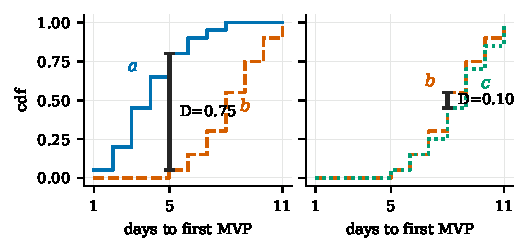
\includegraphics[width=.9\linewidth]{fig/stats_ks}
\caption{The KS statistic is the largest vertical gap between
two cdfs (the black pole).
Left: $a$ versus $b$.
Right: $b$ versus $c$.
Regenerate with \texttt{make statsfig}.}
\label{fig:ks}
\end{figure}
The code walks both sorted lists one distinct value at a time,
advancing two counters \texttt{p} and \texttt{q} past ties, so
the whole pass is linear.
After each advance, \texttt{p/nx} and \texttt{q/ny} are the two
cdfs sampled at the same value \texttt{v}.
Dividing the raw gap by $\sqrt{(n_x+n_y)/(n_x n_y)}$ rescales
it into critical units; at the usual five-percent false-alarm
rate, the \textbf{critical value} on that scale is the tabled
constant $1.36$~\cite{massey51}, so results under $1.36$ are
insignificant.

\begin{lstlisting}[style=py]
def ks(xs, ys):
    nx, ny = len(xs), len(ys)
    d = p = q = 0
    while p < nx and q < ny:
        v = min(xs[p], ys[q])
        while p < nx and xs[p] == v: p += 1
        while q < ny and ys[q] == v: q += 1
        d = max(d, abs(p/nx - q/ny))
    return d / ((nx + ny) / (nx * ny)) ** 0.5
\end{lstlisting}

\subsection{Effect Size}

Two effect sizes are used here: one non-parametric
(Cliff's $\delta$) and one parametric (Cohen's $d$).

\subsubsection{Rank Imbalance: Cliff's $\delta$}

Cliff's $\delta$ is a non-parametric effect
size~\cite{cliff93}.
It asks: if one item is drawn from each sample, how often does
$x$ beat $y$, minus how often $y$ beats $x$?
Naively that is a quadratic all-pairs count.
Sorting first makes it linear: as \texttt{x} ascends, the
counts \texttt{j} and \texttt{k} (how many \texttt{ys} sit
below, and at-or-below, \texttt{x}) only ever move forward.
Romano et al.\ rate $\delta<0.147$ as negligible and
$\delta<0.33$ as small~\cite{romano06}; our threshold of
$0.195$ splits that range, a slightly strict ``smallish.''

\begin{lstlisting}[style=py]
def cliffs(xs, ys):
    gt = lt = j = k = 0
    for x in xs:
        while j < len(ys) and ys[j] < x: j += 1; k = j
        while k < len(ys) and ys[k] == x: k += 1
        gt += j; lt += len(ys) - k
    return abs(gt - lt) / (len(xs) * len(ys))
\end{lstlisting}

\subsubsection{Pragmatic Dullness: Cohen's $d$}

Sooner or later, a business user reviewing statistical results
will say: ``that difference may be real, but it is dull; I only
care about deltas bigger than $x$.''
The complaint bites hardest when results are printed rounded: a
difference can pass both tests above, yet be smaller than the
last digit shown.
Hence one more test is needed, one that can call a difference
real but pragmatically insignificant.
Cohen's $d$ is the standard test for dull: the gap between two
means, in units of the pooled \textbf{standard
deviation}~\cite{cohen88}.
Cohen rated $d\!=\!0.2$ as small and $d\!=\!0.5$ as
medium~\cite{cohen88} (Sawilowsky later refined that
scale~\cite{sawilowsky09}); our threshold of $0.35$ is the
border between the two, so gaps under about a third of a
standard deviation count as dull.
If no such pragmatic argument is needed, set \texttt{c0} to
infinity in \texttt{same} and \texttt{cohen} loses its vote.

The pooled deviation weights each sample's \textbf{variance} by
its degrees of freedom, so unequal sample sizes are handled
fairly.
A \texttt{TINY} constant guards the division when both samples
have near-zero spread.
The code needs no imports: on sorted data, the gap between the
10th and 90th percentile spans 2.56 standard deviations of a
normal curve, so one subtraction estimates the deviation.

\begin{lstlisting}[style=py]
TINY = 1e-32

def mean(a): return sum(a) / len(a)
def stdev(a): n = len(a)//10; return (a[9*n]-a[n])/2.56

def cohen(xs, ys):
    n, m = len(xs), len(ys)
    sd = (((n-1)*stdev(xs)**2 +
           (m-1)*stdev(ys)**2) / (n+m-2)) ** 0.5
    return abs(mean(xs) - mean(ys)) / (sd + TINY)
\end{lstlisting}

\subsection{Ranking Many Treatments}
\label{sec:ranks}

Real studies compare many treatments, not two.
Running all pairwise tests invites false alarms, so instead the
treatments are sorted by their \textbf{medians}, then swept
once from best to worst.
Each treatment is compared to the best member of the current
\textbf{rank}; when \texttt{same} says they are indistinguishable, the
rank is shared, otherwise a new rank opens.
Rank zero holds the winners; the full table maps every
treatment to its rank.
The flag \texttt{big} flips the sort for measures where larger
is better.

\begin{lstlisting}[style=py]
def ranks(d, big=False):
    mid  = lambda t: t[len(t) // 2]
    dd   = {k: sorted(v) for k, v in d.items()}
    out, win, rank, best = {}, [], -1, None
    for k in sorted(dd, key=lambda k: mid(dd[k]), reverse=big):
        if best is None or not same(dd[best], dd[k]):
            rank, best = rank + 1, k
        if rank == 0: win.append(k)
        out[k] = rank
    return win, out
\end{lstlisting}

Applied to the worked example (where fewer days is better, so
\texttt{big} stays false), \texttt{ranks} sorts the frameworks
by their medians (4, 8, 9 days), gives $a$ rank zero, then
finds $b$ and $c$ indistinguishable, so they share rank one.
That is, this data forms two groups:
\begin{center}
\texttt{( (a)~~(b c) )}
\end{center}
and the winners list is just $[a]$.

Note the single sort at the top of \texttt{ranks}: every later
test then runs on pre-sorted lists, so the whole ranking costs
one sort per treatment plus one linear sweep.

Results sections often end with a chart like
Table~\ref{tbl:grid}: here, ten treatments are compared on ten
data sets, twenty runs per cell.
Grey marks the top-ranked treatments of each data set; the
bottom row counts how often each treatment reaches the top
rank.
Such a chart supports a one-sentence summary: rx7 wins over
everything else (but see db2 and db5 for counterexamples).
The result is a statistics stack small enough to audit in an
afternoon, yet defensible enough for a results section.

\begin{table}[!t]
\caption{Ten treatments (rx1..rx10) on ten data sets
(db1..db10).
Cells show the median of twenty runs (fewer is better); grey
cells sit at the top rank of their data set, as computed by
\texttt{ranks}; the bottom row counts top-rank appearances.
Summary: rx7 wins over everything else, but see db2 and db5 for
counterexamples.
Regenerate with \texttt{make statsfig}.}
\label{tbl:grid}
\centering\small
\setlength{\tabcolsep}{2.5pt}
\begin{tabular}{@{}l*{10}{r}@{}}
\toprule
 & rx1 & rx2 & rx3 & rx4 & rx5 & rx6 & rx7 & rx8 & rx9 & rx10\\
\midrule
db1 & 8.2 & 9.7 & 11.1 & 12.0 & 14.5 & 8.0 & \cellcolor{black!15}5.3 & 10.9 & 12.7 & 14.1\\
db2 & 8.4 & \cellcolor{black!15}3.1 & 11.0 & 11.9 & 14.3 & 8.5 & 12.4 & 11.3 & 12.5 & 14.1\\
db3 & 8.7 & 9.7 & 10.9 & 12.4 & 13.8 & 7.9 & \cellcolor{black!15}5.5 & 11.3 & 12.5 & 13.9\\
db4 & 8.2 & 9.6 & 11.0 & 12.7 & 14.0 & 8.0 & \cellcolor{black!15}5.4 & 11.1 & 12.6 & 14.2\\
db5 & 8.3 & 9.2 & 11.3 & 12.7 & \cellcolor{black!15}3.2 & 8.1 & 12.5 & 11.2 & 12.5 & 14.0\\
db6 & 8.1 & 9.7 & 10.9 & 12.5 & 14.2 & 8.4 & \cellcolor{black!15}5.1 & 10.9 & 12.1 & 14.3\\
db7 & 8.2 & 9.7 & 11.2 & 12.7 & 14.3 & 8.3 & \cellcolor{black!15}5.2 & 10.5 & 12.7 & 14.4\\
db8 & 8.4 & 9.5 & 11.3 & 12.7 & 13.7 & 7.8 & \cellcolor{black!15}4.7 & 10.6 & 12.2 & 14.1\\
db9 & 8.1 & 9.5 & 10.7 & 12.5 & 13.7 & 8.2 & \cellcolor{black!15}5.1 & 11.2 & 12.5 & 14.0\\
db10 & 8.5 & 10.0 & 11.1 & 12.5 & 13.9 & 8.5 & \cellcolor{black!15}5.2 & 10.9 & 12.9 & 14.0\\
\midrule
wins & 0 & 1 & 0 & 0 & 1 & 0 & 8 & 0 & 0 & 0\\
\bottomrule
\end{tabular}

\end{table}
